
\pstart  Nota pondus \textit{i} delapsum ex loco in quo pessulo objecto quiescebat ubi follem depresserit, folle abeunte induet se in catenam \protect\index{Sachverzeichnis}{catena}\edtext{uncinatam}{\lemma{catenam}\Afootnote{ \textit{ (1) }\ uncinatam \textit{ (2) }\ capsulatam \textit{ (3) }\ uncinatam \textit{ L}}} pendentem ex rota \textit{tr}. \edtext{Sufficit unum esse uncinum eique a pondere \textit{i} contactu adimi regressum, ac proinde cum catena seu filo attolli, ubi in locum superiorem venerit reddi alicubi contactu libertatem, relabi in locum priorem}{\lemma{\textit{tr.}}\Afootnote{ \textit{ (1) }\ Quae ubi in locum priorem elevaverit \textit{ (2) }\ Sufficit [...] priorem \textit{ L}}}, simulque pondus \textit{i} evertere ac deponere. Id fiet si ei pondus \textit{i} contactu suo claudat foramen vel angustet. Id faciet dum ei pondere suo innitens morderi filum faciet, vel in filo annulum, ita ut se ipsum simul intercludat morsu. Sed \edtext{ubi}{\lemma{}\Afootnote{ubi \textbar\ pondus \textit{i} \textit{ gestr.}\ \textbar\ ascendendum \textit{ L}}} ascendendum erit quod \edtext{pessulum uncini}{\lemma{pessulum}\Afootnote{ \textit{ (1) }\ annuli \textit{ (2) }\ uncini \textit{ L}}} in contrariam partem \edtext{gyrans}{\lemma{gyrans}\Afootnote{\textbar\ annulum \textit{ gestr.}\ \textbar\ deprimendo \textit{ L}}} deprimendo dum attollitur, ac proinde in opposito (quia circa axiculum mobilis) attollendo aperiet et faciet elabi pondus \textso{i}, quo elapso et morsu cessabit, et uncinus delabetur per filum in locum priorem, modo sit ibi extra filum mora, ne descendere ulterius possit, vel sit ibi locus infimus semper fili. 
\pend 
\pstart  Rectius breviusque sic: sit filum vel catena\protect\index{Sachverzeichnis}{catena} (rotae \textit{tr} superioris figurae circumvoluta) \textit{abc} reliquum omne sit pondus \textit{i} superioris figurae demtis \textit{d} et \textit{e}
 %\begin{wrapfigure}{l}{0.6\textwidth}           %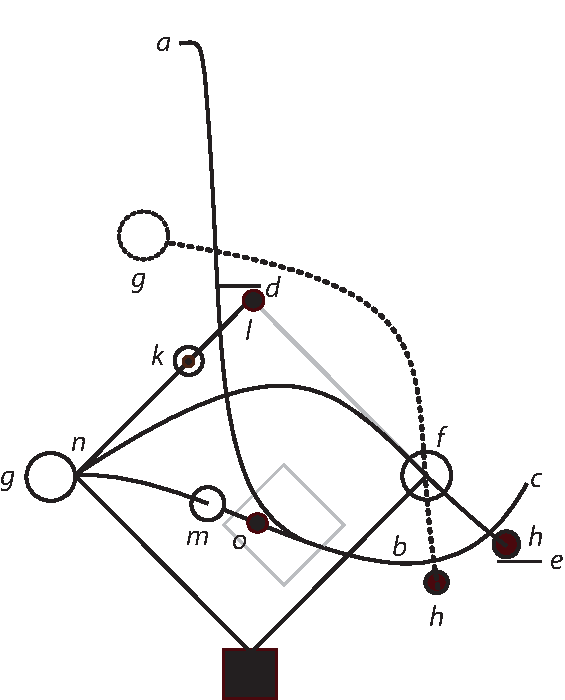
\includegraphics[width=1.0\textwidth]{images/38_202v}
 %\end{wrapfigure}
retinaculis, de quibus mox. Pars ponderis \textit{hfg} si aperta sit, ut in situ punctato, vel etiam magis non possit pondus ea suspendi ex filo. Claudatur ergo, quod ita fiet totum pondus \textit{i} cum annexis descendens super folle incidet \textit{h} punctato in retinaculum \textit{e} atque ita pondus \textit{h} a retinaculo elevabitur, pergente nimirum reliquo pondere et proinde \textit{fg} ex altera parte gyratum circa centrum \textit{f} ex situ punctationis descendet in situm continuitatis ibique in \textit{n} penetrabit \textit{g} per decipulas \textit{omnkl}, et sic clausum, \textit{nf}, abeunte fulcro, folle suspendet ex filo totum pondus, atque ita, cum filo ascendet incidet enim inter fili pinnas. Sed ubi in locum debitum pervenerit muscipulas \textit{nkl} in \textit{l} impinget retinaculo \textit{d}, deprimeturque \textit{l} levabitur \textit{n} aperietur muscipula, et pondus \textit{h} a retinaculo \textit{e} liberum circa centrum \textit{f} attollet \textit{g} aperietque \textit{f} ita pondus supra apertum pendere desinet elabeturque in locum suum. Objici huic machinae potest 1) futurum ut congeletur aqua, 2) ut consumatur. Respondetur (1) plerique omnes motum perennem etiam aquae ope quaesierunt, nemo invenit. (2) Sufficeret praestitisse, quod hactenus nemo, ut motus aliquis vi machinae sibi restituat causam suam, atque ita vi intrinseca\protect\index{Sachverzeichnis}{vis!intrinseca} sit perennis, (3) uti congelabitur frigore, ita et calore aliquando redissolvetur; tunc ergo redibit motus erit ergo perennis, etsi interruptus. Perennis, id est perpetuus, nam originario usu perenne est quod durat \textso{per} totum \textso{annum}, (4) dantur liquores incongelabiles iique aut graves ut \mercury, 

%Zeitz auskommentiert
\includegraphics[width=0.018\textwidth]{images/vitriol}
\textsuperscript{li} etc. In \mercury\ pro plumbo\protect\index{Sachverzeichnis}{plumbum} utendum erit auro\protect\index{Sachverzeichnis}{aurum}. In 
%Zeitzauskommentiert
\includegraphics[width=0.018\textwidth]{images/vitriol}
\textsuperscript{li} suffecerit plumbum\protect\index{Sachverzeichnis}{plumbum}. Sed utrumque plumbum \protect\index{Sachverzeichnis}{plumbum} aurumque \protect\index{Sachverzeichnis}{aurum} vitro obductum esse debet, ne corrodatur aut leves, ut spiritus vini\protect\index{Sachverzeichnis}{spiritus!vini}, in hoc pro ligno utendum est bulla \edtext{clausa}{\lemma{}\Afootnote{clausa \textit{ erg.} \textit{ L}}} aere plena. 
(5) Impediri potest aquae congelatio, non
  %\begin{center}
  %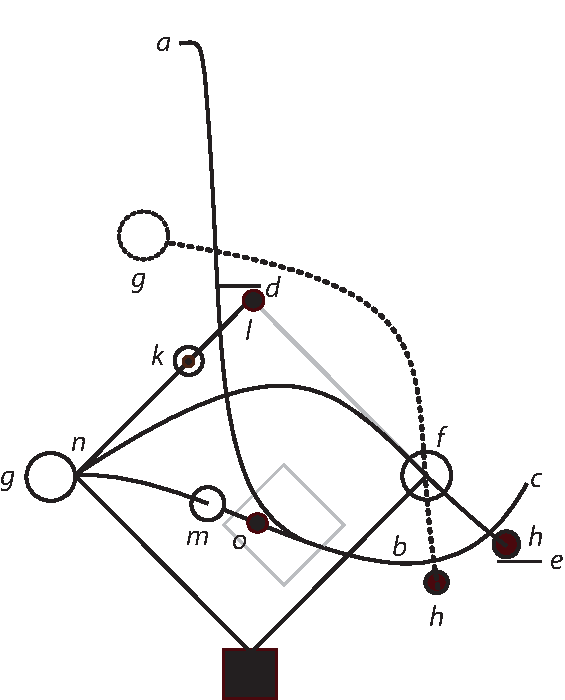
\includegraphics[width=0.75\textwidth]{images/38_202v}\\
  %\vspace{0.5ex}
  %\textit{[Fig. 1]}
  %\vspace{0.5ex}
  %\end{center} 
tantum in hypocaustis sed et in liberrimo aere. Id ita fiet: Constat quicquid congelascit prius tenui crustula vestiri. Quae si perpetuo ab astante aliquo rumperetur, nunquam aqua congelasceret. Id pro astante faciet ipsa machina. Canalis enim aqua eminens perpetuo motus spatium per quod sibi decurrendum est, salvum praestabit, servabitque sibi jus aperturae. Nam si hic liber maneat etsi latera et superficies caeteroquin concrescant, nihil \edtext{motui}{\lemma{nihil}\Afootnote{ \textit{ (1) }\ ad rem \textit{ (2) }\ motui \textit{ L}}} obstat. Aquae enim intima non congelascunt, sed tantum quibus latera tangit, aeremve. Imo efficiemus ut non praecise suum tantum spatium sed et totam pene aquae extremitatem, minimam superficiem praeservet, si reticulus per eam expansus \edtext{tactusque}{\lemma{expansus}\Afootnote{ \textit{ (1) }\ ab eaque \textit{ (2) }\ tactusque \textit{ L}}} motu ac commotus crustulam perpetuo rumpat. (6) At aqua consumetur magis etiam spiritus vini\protect\index{Sachverzeichnis}{spiritus!vini} imo et \mercury, sole vel calore extrahente. Respondeo in forma minore \edtext{et majore}{\lemma{}\Afootnote{et majore \textit{ erg.} \textit{ L}}} hoc impediri in majore reparari potest. Reparabitur, si vicissim ita apertum sit os vasis, ut aquam pluviam hauriat, et in abundanti reponat, suffectura in casum deplementi impedietur vitro hermetice sigillato, si intus sit tota machina intra aquam vel ut si pendulum\protect\index{Sachverzeichnis}{pendulum} esse velimus, intra vas in aere spectabilis. Si vero agere extrorsum aliquid debet, si intus aliquid agi, effici potest magnete\protect\index{Sachverzeichnis}{magnes} in aqua ubi conservatur vel cum canali supra, ut crebro redemergatur extremitati applicato et ita ferrum\protect\index{Sachverzeichnis}{ferrum} exterius applicatum movente. Pone nos in ipsa machina non aperta (quod alioqui facile) aliquid corrigere velle, ut das pendulum\protect\index{Sachverzeichnis}{pendulum} adjoustiren fiet magnete\protect\index{Sachverzeichnis}{magnes} exterius applicato.
\pend \newpage
  \begin{center}
   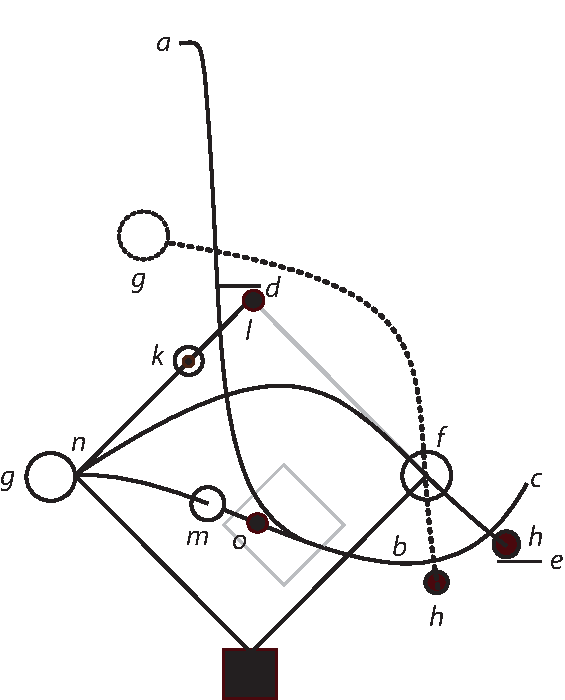
\includegraphics[width=0.75\textwidth]{images/38_202v}\\
   \vspace{0.5ex}
   \textit{[Fig. 1, tlw. Blindzeichnungen]}
   \vspace{1.0ex}
   \end{center} 